% Fig. 1 of the TKDE version: generate -> select -> certify, with the Theorem-2 calibration link.
% Stage 3O: redrawn so that ALL lettering is 8 pt at final size (IEEE's floor for figure text);
% the Stage-3D drawing used 5.6-6.4 pt. Drawn at exactly \textwidth (517.9 pt = 18.20 cm, border 0)
% and included 1:1. To afford 8 pt the box texts were cut to two or three short lines with explicit
% breaks (auto-wrapping had pushed boxes onto each other), and every label that sat inside a
% mini-plot was moved to the line beneath it. Palette shared with figs_tkde.py.
\documentclass[border=0pt]{standalone}
\usepackage{helvet}\renewcommand{\familydefault}{\sfdefault}
\usepackage{amsmath,amssymb}\usepackage{sansmath}\sansmath
\usepackage{tikz}
\usetikzlibrary{positioning,arrows.meta,backgrounds,fit,calc}
\definecolor{ours}{HTML}{0072BD}
\definecolor{oursd}{HTML}{00406A}
\definecolor{cal}{HTML}{7E2F8E}
\definecolor{warn}{HTML}{A2142F}
\definecolor{gry}{HTML}{8C8C8C}
\definecolor{ink}{HTML}{2B2B2B}
\definecolor{lane}{HTML}{F4F7F7}
\newcommand{\md}{\fontsize{8}{9.7}\selectfont}
\begin{document}
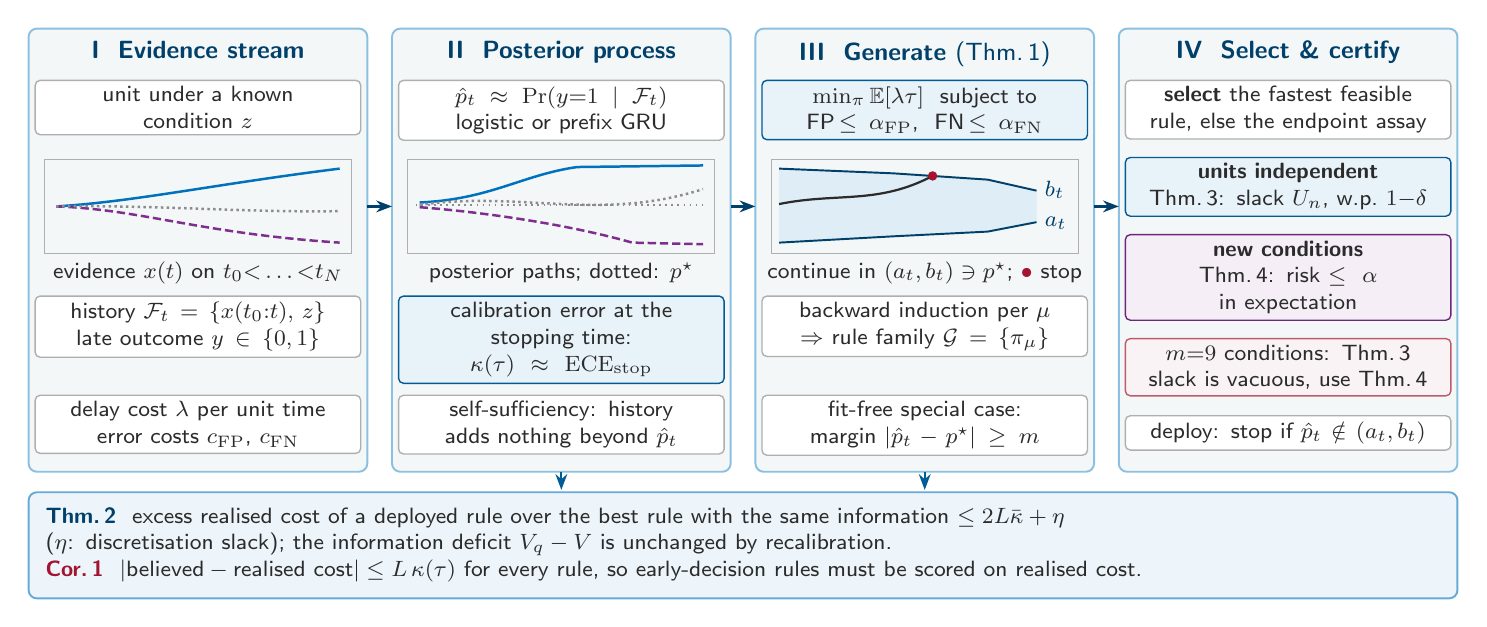
\begin{tikzpicture}[
  font=\md, >={Stealth[length=2.0mm,width=1.5mm]},
  hdr/.style={font=\fontsize{9}{10.8}\selectfont\bfseries, text=oursd, inner sep=0pt},
  box/.style={draw=gry!70, line width=0.5pt, rounded corners=1.8pt, fill=white, align=center,
              inner sep=2.2pt, text=ink, text width=3.98cm},
  tbox/.style={box, draw=ours!80!black, fill=ours!9},
  cbox/.style={box, draw=cal!85!black, fill=cal!8},
  wbox/.style={box, draw=warn!70, fill=warn!5},
  capt/.style={font=\md, text=ink, inner sep=0pt},
  ar/.style={->, line width=0.8pt, draw=oursd},
]
\def\W{4.325}\def\G{0.29}\def\ytop{7.26}\def\ybot{1.62}\def\ymid{4.99}
\path[use as bounding box] (0,0) rectangle (4*\W+3*\G,\ytop);
\foreach \i/\ttl in {0/{I\ \ Evidence stream}, 1/{II\ \ Posterior process},
                     2/{III\ \ Generate \textnormal{(Thm.\,1)}}, 3/{IV\ \ Select \& certify}}{
  \pgfmathsetmacro\xl{\i*(\W+\G)}
  \fill[lane,rounded corners=3pt,draw=ours!45,line width=0.7pt] (\xl+0.012,\ybot) rectangle (\xl+\W-0.012,\ytop-0.012);
  \node[hdr,anchor=north] at (\xl+\W/2,\ytop-0.17) {\ttl};
}
% ------------------------------------------------ I evidence stream
\begin{scope}[shift={(0,0)}]
  \node[box,anchor=north] at (\W/2,6.60) {unit under a known\\ condition $z$};
  \begin{scope}[shift={(\W/2,\ymid)}]
    \draw[gry!70,line width=0.4pt] (-1.95,-0.60) rectangle (1.95,0.60);
    \draw[ours,line width=0.9pt] (-1.8,0.0) .. controls (-0.8,0.06) and (0.2,0.28) .. (1.8,0.48);
    \draw[cal,line width=0.9pt,dash pattern=on 3pt off 1.4pt] (-1.8,0.0) .. controls (-0.7,-0.04) and (0.0,-0.34) .. (1.8,-0.46);
    \draw[gry,line width=0.9pt,dash pattern=on 0.9pt off 1.2pt] (-1.8,0.0) .. controls (-0.5,0.02) and (0.6,-0.08) .. (1.8,-0.06);
  \end{scope}
  \node[capt] at (\W/2,4.15) {evidence $x(t)$ on $t_0{<}\dots{<}t_N$};
  \node[box,anchor=north] at (\W/2,3.86) {history $\mathcal F_t=\{x(t_0{:}t),\,z\}$\\ late outcome $y\in\{0,1\}$};
  \node[box,anchor=north] at (\W/2,2.60) {delay cost $\lambda$ per unit time\\ error costs $c_{\rm FP}$, $c_{\rm FN}$};
\end{scope}
% ------------------------------------------------ II posterior process
\begin{scope}[shift={(\W+\G,0)}]
  \node[box,anchor=north] at (\W/2,6.60) {$\hat p_t\approx\Pr(y{=}1\mid\mathcal F_t)$\\ logistic or prefix GRU};
  \begin{scope}[shift={(\W/2,\ymid)}]
    \draw[gry!70,line width=0.4pt] (-1.95,-0.60) rectangle (1.95,0.60);
    \draw[gry,line width=0.5pt,dash pattern=on 0.6pt off 1.6pt] (-1.85,0.02)--(1.85,0.02);
    \draw[ours,line width=0.9pt] (-1.8,0.05) .. controls (-0.9,0.09) and (-0.5,0.40) .. (0.2,0.50) -- (1.8,0.52);
    \draw[cal,line width=0.9pt,dash pattern=on 3pt off 1.4pt] (-1.8,-0.01) .. controls (-0.8,-0.09) and (0.2,-0.26) .. (0.9,-0.46) -- (1.8,-0.48);
    \draw[gry,line width=0.9pt,dash pattern=on 0.9pt off 1.2pt] (-1.8,0.02) .. controls (-0.5,0.20) and (0.5,-0.20) .. (1.8,0.22);
  \end{scope}
  \node[capt] at (\W/2,4.15) {posterior paths; dotted: $p^\star$};
  \node[tbox,anchor=north] at (\W/2,3.86) {calibration error at the\\ stopping time:\\ $\kappa(\tau)\approx\mathrm{ECE}_{\rm stop}$};
  \node[box,anchor=north] at (\W/2,2.60) {self-sufficiency: history\\ adds nothing beyond $\hat p_t$};
\end{scope}
% ------------------------------------------------ III generate
\begin{scope}[shift={(2*\W+2*\G,0)}]
  \node[tbox,anchor=north] at (\W/2,6.60) {$\min_\pi\mathbb E[\lambda\tau]$\ \ subject to\\ FP$\,\le\alpha_{\rm FP}$,\ \ FN$\,\le\alpha_{\rm FN}$};
  \begin{scope}[shift={(\W/2,\ymid)}]
    \draw[gry!70,line width=0.4pt] (-1.95,-0.60) rectangle (1.95,0.60);
    \fill[ours!13] (-1.85,-0.46) -- (-0.4,-0.38) -- (0.8,-0.32) -- (1.42,-0.20) -- (1.42,0.20) -- (0.8,0.34) -- (-0.4,0.42) -- (-1.85,0.48) -- cycle;
    \draw[oursd,line width=0.7pt] (-1.85,0.48) -- (-0.4,0.42) -- (0.8,0.34) -- (1.42,0.20);
    \draw[oursd,line width=0.7pt] (-1.85,-0.46) -- (-0.4,-0.38) -- (0.8,-0.32) -- (1.42,-0.20);
    \node[text=oursd,anchor=west,font=\md,inner sep=0pt] at (1.52,0.21) {$b_t$};
    \node[text=oursd,anchor=west,font=\md,inner sep=0pt] at (1.52,-0.21) {$a_t$};
    \draw[ink,line width=0.8pt] (-1.85,0.03) .. controls (-1.1,0.18) and (-0.6,0.02) .. (0.1,0.387);
    \fill[warn] (0.1,0.387) circle (0.6mm);
  \end{scope}
  \node[capt] at (\W/2,4.15) {continue in $(a_t,b_t)\ni p^\star$; \textcolor{warn}{$\bullet$} stop};
  \node[box,anchor=north] at (\W/2,3.86) {backward induction per $\mu$\\ $\Rightarrow$ rule family $\mathcal G=\{\pi_\mu\}$};
  \node[box,anchor=north] at (\W/2,2.60) {fit-free special case:\\ margin $|\hat p_t-p^\star|\ge m$};
\end{scope}
% ------------------------------------------------ IV select & certify
\begin{scope}[shift={(3*\W+3*\G,0)}]
  \node[box,anchor=north] at (\W/2,6.60) {\textbf{select} the fastest feasible\\ rule, else the endpoint assay};
  \node[tbox,anchor=north] at (\W/2,5.62) {\textbf{units independent}\\ Thm.\,3: slack $U_n$, w.p.\ $1{-}\delta$};
  \node[cbox,anchor=north] at (\W/2,4.64) {\textbf{new conditions}\\ Thm.\,4: risk $\le\alpha$\\ in expectation};
  \node[wbox,anchor=north] at (\W/2,3.32) {$m{=}9$ conditions: Thm.\,3\\ slack is vacuous, use Thm.\,4};
  \node[box,anchor=north] at (\W/2,2.34) {deploy: stop if $\hat p_t\notin(a_t,b_t)$};
\end{scope}
% ------------------------------------------------ flow arrows
\foreach \i in {1,2,3}{\pgfmathsetmacro\xa{\i*(\W+\G)-\G}\draw[ar] (\xa-0.012,\ymid) -- (\xa+\G+0.012,\ymid);}
% ------------------------------------------------ Theorem 2 strip
\pgfmathsetmacro\xr{4*\W+3*\G}
\fill[ours!7,rounded corners=3pt,draw=ours!60,line width=0.7pt] (0.012,0.012) rectangle (\xr-0.012,1.36);
\node[font=\md,text=ink,anchor=west,text width=17.72cm,align=left,inner sep=0pt] at (0.22,0.69)
  {\textbf{\textcolor{oursd}{Thm.\,2}}\ \ excess realised cost of a deployed rule over the best rule with the same information
   $\le 2L\bar\kappa+\eta$\\ ($\eta$: discretisation slack); the information deficit $V_q-V$ is unchanged by recalibration.\\
   \textbf{\textcolor{warn}{Cor.\,1}}\ \ $|\text{believed}-\text{realised cost}|\le L\,\kappa(\tau)$ for every rule, so
   early-decision rules must be scored on realised cost.};
\draw[->,line width=0.7pt,draw=ours!80!black,dashed] (\W+\G+\W/2,\ybot) -- (\W+\G+\W/2,1.39);
\draw[->,line width=0.7pt,draw=ours!80!black,dashed] (2*\W+2*\G+\W/2,\ybot) -- (2*\W+2*\G+\W/2,1.39);
\end{tikzpicture}
\end{document}
